\documentclass[fontsize=11pt,paper=a4,]{scrartcl}

% use pdflatex to compile the document!
% Compile the report from this file (TEMPLATE.tex), using the following sequence:
%		a. PDFLaTex
%		b. BibTex
%		c. PDFLaTex
%		d. PDFLaTex

\usepackage[english]{babel}
\usepackage[margin=3cm]{geometry}
\usepackage[T1]{fontenc}
\usepackage[utf8]{inputenc}
\usepackage{lmodern}
\usepackage{graphicx}
\usepackage{fancyhdr}
\usepackage[textfont={small,it},labelfont=bf,labelsep=endash]{caption}
\usepackage[table]{xcolor}
\usepackage{verbatim}
\usepackage[toc,page]{appendix}
\usepackage{amssymb} % Mathematical Symbols
\usepackage{amsmath}
\usepackage{multicol}	% allow multi column environemnt
%\usepackage{mathtools}
%\usepackage[framed,numbered]{mcode}
\usepackage{acronym}
\usepackage{rotating}
\usepackage{titling}
\usepackage{bibcheck}
%\usepackage{pdfpages}
%\usepackage[pdfpagemode=FullScreen,pdfstartview=FitH,pdfborder={0 0 0},pdftitle={My report},bookmarks,pdfauthor={Morten Olsen}]{hyperref}
\usepackage{memhfixc}
%\usepackage{maplestd2e}
\addtokomafont{disposition}{\boldmath} % bold math text in section names
\usepackage{lipsum}
\usepackage{placeins} % provides \FloatBarrier to keep floats in right chapter
\usepackage{geometry} % Allow changing of page margin
\usepackage{textcomp}


%Bibliography 
% You need biblatex-package. Ubuntu: sudo apt-get install biblatex
\usepackage[style=numeric-comp]{biblatex}
\bibliography{library.bib}

% Colors & Links
\usepackage{color, xcolor}
\usepackage[pdftex]{hyperref} % Enable hyperlinks
\hypersetup{colorlinks=true,
linkcolor=black,
citecolor=black,
filecolor=black,
urlcolor=black,
pdftitle={UniSpace -- Imaging Subsystem PDR}}

\newcommand{\unit}[1]{\ensuremath{\,\mathrm{#1}}}
\newcommand{\degr}{\ensuremath{^\circ}}
\newcommand{\cel}{\ensuremath{\degr\mathrm{C}}}
\newcommand{\dif}{\ensuremath{\mathrm{d}}}
\newcommand{\ee}[1]{\ensuremath{\cdot 10^{#1}}}



\definecolor{tableshade}{HTML}{E8E8E8}
\linespread{1.3}


\fancyhead{}
\fancyhead[RE,RO]{\parbox[b]{10cm}{\raggedleft U-SPACE\\ \today}}
\fancyhead[LE,LO]{\parbox[b]{10cm}{\docreference \\ \title }}
\renewcommand{\headrulewidth}{0.4pt}
\fancyhfoffset{1cm}
\addtolength{\headheight}{1cm}
\fancyfoot{}
\fancyfoot[C]{\thepage}
\renewcommand{\footrulewidth}{0.4pt}


\graphicspath{{figures/}}


% more space for graphics on each page
\renewcommand{\topfraction}{1}
\renewcommand{\bottomfraction}{1}
\renewcommand{\textfraction}{0.1}

% formatting options
\setlength{\parindent}{0pt}
\setlength{\parskip}{0.5\baselineskip}
\pagestyle{fancy}
\fancyhead[RH]{UniSpace imaging subsystem PDR}



\def\authors{
Bastian \textsc{Hacker}\\
Oliver \textsc{Porges}\\
Omair \textsc{Sarwar}\\
Jan \textsc{Sommer}
}
\def\docversion{DRAFT}					% Possible versions are: DRAFT, REVIEW or RELEASED
\def\docreference{USPACE-PDR-imaging~payload-00}	% -00 = DRAFT,  -A1 = 1st release,  -A2 = 1st release with minor updates, -B1, = 2nd release
\def\title{Preliminary Design Report}
\def\subtitle{imaging subsystem}


\begin{document}
\sloppy

\begin{titlepage}

\begin{center}


\includegraphics[width=0.6\textwidth]{figures/logo.pdf}\\[0.75cm] 

\textsc{\large Unmanned Solar Powered Airship Concept Evaluation}\\[1cm]

\line(1,0){415}\\[1mm]
\vspace{-1.0em}
\Huge \bfseries{\title}\\[2mm] 
\LARGE \bfseries{\subtitle}\\
%\
\vspace{-1.0em}
\line(1,0){415}\\[1cm]

\begin{large}
\begin{tabular}{ll}
Document Reference No.: & \docreference\\[5mm]
Document Status: & \docversion \\[1.5cm]
\end{tabular}
\end{large}

\begin{minipage}[t]{0.49\textwidth}
\begin{flushleft} \large
\emph{Authors}\\
\vspace{-1.2em}
\line(1,0){125}\\
\authors
\end{flushleft}
\end{minipage}
\begin{minipage}[t]{0.49\textwidth}
\begin{flushright} \large
\emph{Supervisors}\\
\vspace{-1.2em}
\line(1,0){125}\\
Kjell \textsc{Lundin}\\
Alf \textsc{Wikstr\"{o}m}
\end{flushright}
\end{minipage}

\vspace{1cm}

\begin{minipage}[t]{0.49\textwidth}
\begin{flushleft} \large
\emph{Project Manager}\\
\vspace{-1.2em}
\line(1,0){125}\\
Dries \textsc{Agten}
\end{flushleft}
\end{minipage}
\begin{minipage}[t]{0.49\textwidth}
\begin{flushright} \large
\emph{Quality Manager}\\
\vspace{-1.2em}
\line(1,0){125}\\
Morten \textsc{Olsen}\\[1cm]
\end{flushright}
\end{minipage}

\vfill

\begin{large}
\today \\
Lule\r{a} University of Technology \\
Rymdcampus, Kiruna, Sweden\\
\end{large}

\end{center}

\end{titlepage}

\pagestyle{plain}
\pagenumbering{roman}

\thispagestyle{plain}
\section*{Acronyms}
\markboth{Acronyms}{Acronyms}
\addcontentsline{toc}{section}{\protect\numberline{}Acronyms}

\begin{multicols}{2}
\begin{acronym}
\acro{APR}{Array Power Regulator}
\acro{B2R}{Buck-Boost Regulator}
\acro{BCR}{Battery Charge Regulator}
\acro{BDR}{Battery Discharge Regulator}
\acro{BJT}{Bipolar Junction Transistor}
\acro{BoIBB}{Boost Interleaved By Buck}
\acro{BoSBB}{Boost Superimposed By Buck}
\acro{BuCBB}{Buck Cascaded By Boost}
\acro{CCM}{Continuous Conduction Mode}
\acro{CM}{Current Mode}
\acro{DCM}{Discontinuous Conduction Mode}
\acro{DET}{Direct Energy Transfer}
\acro{ECSS}{European Cooperation for Space Standardization}
\acro{EMI}{Electromagnetic Interference}
\acro{EOL}{End Of Lifetime}
\acro{EPS}{Electrical Power Subsystem}
\acro{ESA}{European Space Agency}
\acro{ESR}{Equivalent Series Resistor}
\acro{GaAs}{Gallium Arsenide}
\acro{IC}{Integrated Circuit}
\acro{IRF}{International Rectifiers}
\acro{LEO}{Low Earth Orbit}
\acro{LT}{Linear Technology}
\acro{MDC}{Mode Detection Circuit}
\acro{MEA}{Main Error Amplifier}
\acro{MPP}{Maximum Power Point}
\acro{MPPT}{Maximum Power Point Tracking}
\acro{MPPTU}{Maximum Power Point Tracking Unit}
\acro{OpAmp}{Operational Amplifier}
\acro{PCB}{Printed Circuit Board}
\acro{PCU}{Power Conditioning Unit}
\acro{PWM}{Pulse Width Modulated}
\acro{PFC}{Power Factor Corrector}
\acro{PI}{Proportional-Integral}
\acro{PV}{Photo Voltaic}
\acro{RHPZ}{Right Half Plane Zero}
\acro{S3R}{Sequential Switch Shunt Regulator}
\acro{SA}{Solar Array}
\acro{SEE}{Single Event Effect}
\acro{SSA}{State Space Averaging}
\acro{TI}{Texas Instruments}
\end{acronym}
\end{multicols}



\markboth{List of Figures}{List of Figures}
\addcontentsline{toc}{section}{\protect\numberline{}List of Figures}
\listoffigures
\newpage

\markboth{List of Tables}{List of Tables}
\addcontentsline{toc}{section}{\protect\numberline{}List of Tables}
\listoftables
\newpage

\tableofcontents
\newpage
\acresetall	%reset acronyms which is otherwise used in list of figures or tables
\clearpage %reset page numbers
\pagenumbering{arabic}
\pagestyle{fancy}




\section{Subsystem Introduction}
The Imaging Payload Subsystem (IPS) is the scientific payload of the airship, and will be independent of the airship project to a large extent.
The purpose of IPS is to take aerial images from different positions, acquire accurate position and attitude data and use those combined information to create aerial image maps and extract further information from the images such as terrain height, 3D object recognition and possibly image-aided attitude control and path planning.
This could be used as a learning platform to simulation environment for Low Earth Orbit imaging.

The system is further divided into the following parts:
\begin{itemize}
\item Attitude determination: Usage of advanced data fusion method to facilitate GPS, Gyro, Accelerometer and Magnetometer information, to extract accurate position and attitude information together with reasonable error estimates.
\item Imaging system: A megapixel resolution webcam will provide images in regular timesteps in the order of a second.
The image data will be saved on a SD memory card together with attitude information for offline processing.
\item Communication system: Attitude data and possibly spacecraft telemetry will be transmitted to ground.
We try to achieve high bandwidth transmission that could even allow for image downlink.
\item Image processing software:
Image matching and evaluation will be done on a standard PC after payload recovery or online if the transmission rate can be made sufficient.
There will also be a groundstation that communicates with the spacecraft during flight.
\end{itemize}


\section{Technical and functional requirements}
\subsection{Functional requirements}
\label{sub:Functional_requirements}
\begin{itemize}
\item Measure absolute and accurate position and pointing angles.
\item Take images in regular steps and save them together with attitude data.
\item Receive and execute basic telecommands such as image capture start/stop.
\item Send basic telemetry data such as position.
\item Combine single image captures to a large area map.
\end{itemize}


\subsection{Technical requirements}
\begin{itemize}
\item Operate in open air environment up to 800m over ground.
\item Operate at 5V unstabilized input voltage at a maximum power consumption of 2.5W.
\item Store at least 1000 medium-resolution images.
\end{itemize}


\subsection{Expected performance}
\begin{itemize}
\item Operate in image capture mode for at least 15 minutes.
\item Create aerial images with 10cm horizontal resoultion (pixel size).
\item Optional: Extract height information with 0.5m relative and 7m absolute resulution.
\end{itemize}

\section{Preliminary Design}

\subsection{Electronic components}
In this section an overview about the requirements and the planned electronic components is given. In order to achieve the functional requirements mentioned in \ref{sub:Functional_requirements} following components are needed:

\begin{itemize}
 \item Board computer
 \item Accelerometer
 \item Magnetometer
 \item Gyroscope
 \item GPS-receiver
 \item Transmitter/Receiver
 \item Camera
\end{itemize}


\subsubsection*{Board computer}

For controlling the sensors and the camera as well as communicating with the ground station first a standard microcontroller was considered, but as the requirements in \ref{sub:Functional_requirements} state, it is necessary to get a picture around every second. Also the resolution of the pictures should be in the range of some megapixels. Taken this into account, a standard microcontroller would not be able to process these amounts of data fast as well as it normally does not come with a USB-interface necessary for connecting most cameras.

Instead it was decided to use a BeagleBone embedded computer \cite{BeagleBone:SRM}. It is populated with an ARM Cortex-A8 microprocessor running at 500 -- 700 MHz and provides an USB-port, several I{\texttwosuperior}C and serial interfaces. It is capable of running an embedded Linux operation system and therefore able to support a large varity of devices (plugged to the USB-port) and to provide the possibility for sophisticated onboard calculations from a large set of libraries.

\subsubsection*{Sensors}

For sensors it is planned to use the LSM303 \cite{LSM303:datasheet} combined magnetometer and accelerometer and the ITG-3200 triple-axis gyroscope \cite{ITG-3200:datasheet} from sparkfun. Both sensors have been used during the CanSat-project in Würzburg, hence the group is familiar with working with this sensors. They communicate via an I{\texttwosuperior}C interface with the main board. For receiving GPS information a LS20031 5~Hz GPS receiver \cite{LS20031:datasheet} can be used. It is connected via a serial line interface with the main board.


\subsubsection*{Transmitter/Receiver}
WiFi - long range antenna?


\subsubsection*{Camera}

As high quality embedded industrial cameras are very high priced it is planned to connect a consumer webcam with a resolution of several megapixels to the USB-port of the main board. It is intended to buy a camera which is supported by the Linux operating system running on the main board. To save weight, the case of the webcam will be stripped as much possible leaving only the bare camera and electronics. An example of a compatible camera would be the Logitech HD Webcam C525\footnote{\url{http://www.logitech.com/de-de/webcam-communications/webcams/devices/7794}}.


\FloatBarrier
\subsection{Attitude Determination System}
The Attitude Determination System (ADS) measures and estimates position and pointing direction of the payload system.
This is crucial for the further use of recordet images, as it provides the reference system and relative alignment of the taken images towards each other.
\begin{figure}
\centering
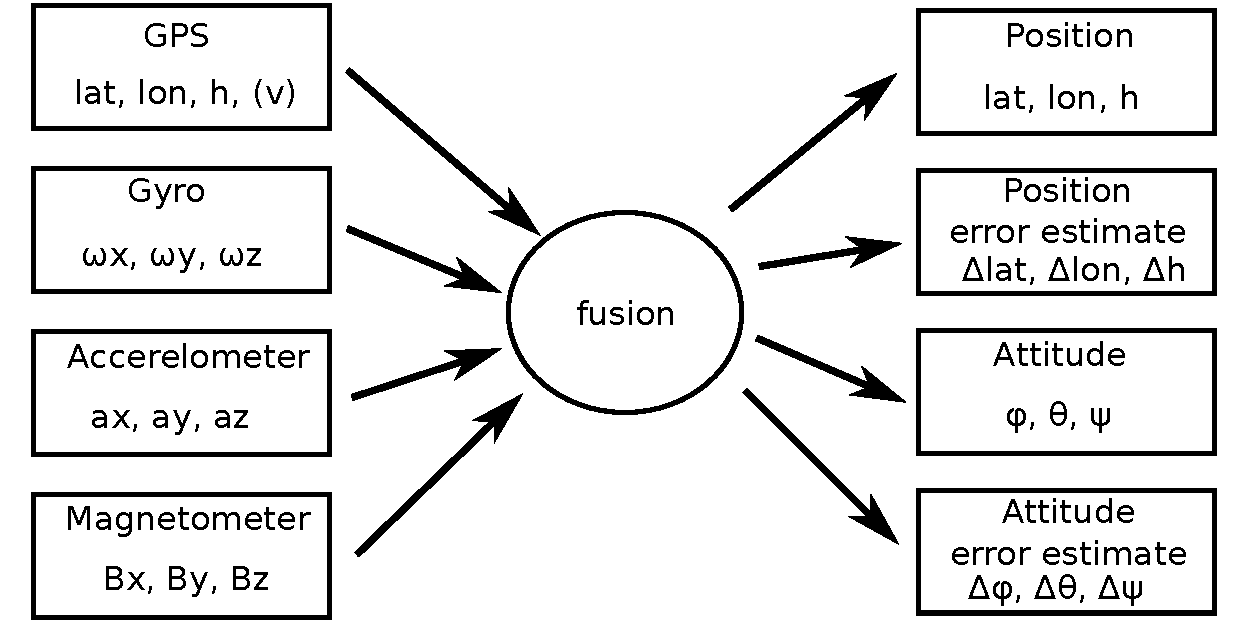
\includegraphics[width=0.8\textwidth]{figures/ADS_diagram.pdf}
\caption{Attitude Determination System overview}
\label{fig:ADS_overview}
\end{figure}

In order to produce high-accuracy attitude estimates and compensate for disadvantages of certain sensor types such as drift and noise, we chose to use a variety of sensors and fuse their information to a combined information.
The facilitated sensors will be (\ref{fig:ADS_overview}):
\begin{itemize}
\item GPS receiver: Provides absolute position values, but has much high-frequency noise
\item Gyroscope: Provides accurate relative pointing direction, but has drift.
\item Accerelometer: Provides absoulte pointing relative to the horizon (gravity) and linear acceleration.
\item Magnetometer: Provides absolute pointing relative to the earth's magnetic field.
\end{itemize}

Combined all together, these sensors provide complete information about the module's attitude.
As a fusion method we will use well-understood algorithms, such as the extended Kalman filter.

The fused information will be updated in real-time and stored together with each image snapshot.


\FloatBarrier
\subsection{Software environment}
Since a Linux operating system is run as a basic software layer, it is planned to deploy the Robot Operating System (ROS) as a middle-ware. This system is a modern framework
for mobile robotic applications. Its main advantage is the interoperability of modules and inter-use of underlying 
layers. This increases the flexibility of future research and overall system robustness. Since ROS is an open-source system along with its packages it is used for knowledge exchange and achievement demonstration in terms of modern algorithms. These algorithms include Simultaneous Localization
And Mapping (SLAM), Navigation and position control, Image processing and many more.  

\subsection{Image processing}
The main goal is to take numerous aerial images and combine them into one usable map. This system should then be able
to automatically collect images over a given area and produce an aerial map. A proposed solution
for image matching is described in section ~\ref{sec:algorithm}

\subsubsection*{Image matching}
\label{sec:algorithm}
The proposed solution should be very robust to different illumination conditions and overall image quality, namely sharpness. 
\begin{enumerate}
\item Step\\
It is needed to extract common and significant points from all the images in question. Since the images
will be taken in sequence it can be assumed that there will be a high correlation in the neighboring pictures.
Having this assumption an algorithm proposed in [bib-ref] can be implemented for finding 
Points of Interest (POI) based on histogram leveling. 
\item Step \\
Having a reliable set of POI another technique to match the points together can be used. This part is
computationally intensive. In order to be able to use it in real-time it is recommended to use the Iterative Closest Point
algorithm already implemented and optimized in the Point Cloud Library[bib-ref].
\item Step\\
By knowing the difference between two set of points in two consecutive images it is possible to calculate
a very precise transformation matrix. The transformation will be determined by how many points
could be found in the previous step. The expectation in a general scenery and medium resolution picture
is about a 100 points. This would be enough even to compensate for camera deformation.
\item Step \\
As a last step the transformation matrix obtained before has to be applied to the images before combining them into one large array. 
\end{enumerate}


\FloatBarrier
\section{Test and Verification of Design}
???


\section{Resources and Scheduling}
\subsection{Main Tasks}
\subsection{Parts List and Costs}
\subsection{Electronics Ground Support Equipment (EGSE)}
\subsection{Mechanical Ground Support Equipment (MGSE)}


\section{Discussions/Questions}

I (Jan) will take {\color{green} a green color}:

{\color{green} So what kind of sections are missing? Here what came to my mind:
\begin{itemize}
 \item Budget
 \item Power-Budget
 \item Something about the how of sensor fusion?
 \item Something about the how of image processing?
\end{itemize}
}


\newpage
\printbibliography
\markboth{Bibliography}{Bibliography}
\addcontentsline{toc}{section}{\protect\numberline{}References}
\pagestyle{plain}

\end{document}
